\chapter{S-Parameters}
    \textbf{S-Parameters} là một công cụ có giá trị để tính toán 
    \textbf{hệ số phản xạ} (reflection coefficient) và \textbf{độ lợi truyền dẫn} (transmission gain)
    cho các đầu vào và đầu ra của mạng hai cổng. 
    Khái niệm cơ bản này xác định tham số S cho 
    mạng nhiều cổng, tính toán các tham số như 
    \textit{return loss}, \textit{VSWR} và 
    \textit{insertion loss}. 
    Trong bối cảnh này, thuật ngữ tham số S hay 
    tham số "tán xạ" đề cập đến cách dòng điện hoặc 
    điện áp di chuyển bị ảnh hưởng khi chúng gặp sự 
    cố trên đường truyền.

    \section{Định nghĩa S-parameters}
        Ma trận tham số S cho mạng 2 cổng là thành phần cơ bản để xây dựng các ma trận bậc cao hơn cho các mạng mở rộng hơn. 
        Mối quan hệ giữa sóng đi ra (sóng phản xạ) và sóng tới và ma trận tham số S có thể được biểu thị 
        trong công thức sau và nhân với nhau để có được các phương trình riêng cho $b_1$ và $b_2$.
        \cite{cadence2023sparams}
        \begin{equation}
            \begin{bmatrix}
                b_1 \\
                b_2
            \end{bmatrix}
                =
            \begin{bmatrix}
                S_{11} & S_{12} \\
                S_{21} & S_{22}
            \end{bmatrix}
            \begin{bmatrix}
                a_1 \\
                a_2
            \end{bmatrix}
        \end{equation}
        \begin{itemize}
            \item $a_i$: Sóng tới tại cổng $i$
            \item $b_i$: Sóng phản xạ tại cổng $i$
            \item $S_{ii}$: Hệ số phản xạ tại cổng $i$
            \item $S_{ij}$: Hệ số truyền dẫn từ cổng $i$ đến cổng $j$
        \end{itemize}

        \subsection{S-Parameters trên thang đo decibel (dB)}
            $S_{11}$ biểu thị tổn thất phản hồi của một thiết bị, 
            cho biết lượng công suất đầu vào được cung cấp cho thiết bị 
            phản xạ trở lại cổng đầu vào. 
            Lý tưởng nhất là không nên có công suất phản xạ và 
            100\% công suất phải được cung cấp cho thiết bị.\par

            Khi $S_{11}$ ở mức -10 dB, điều đó có nghĩa là ít nhất 90\% 
            công suất đầu vào được truyền hiệu quả đến thiết bị, 
            với ít hơn 10\% bị phản xạ.

    \section{Trở kháng đầu vào (Input Impedance)}
        Trở kháng đầu vào (Zin) là trở kháng mà nguồn nhìn thấy khi tín hiệu đi vào đường truyền.
        \begin{equation}
            Z_{in} = Z_0 \frac{Z_L + Z_0 \tanh(\gamma l)}{Z_0 + jZ_L \tanh(\gamma l)}
            \label{eq:zin}    
        \end{equation}
        
        \begin{itemize}
            \item $l$: Chiều dài đường truyền
        \end{itemize}

    \section{S11 (Return Loss)}
        Định nghĩa về return loss theo hệ số phản xạ đường truyền.
        $$RL = -10\log\left(\left|\frac{P_{ref}}{P_{inc}}\right|\right) = -20\log\left(\left|\frac{V_{ref}}{V_{inc}}\right|\right) = -20\log\left(\left|\Gamma\right|\right)$$
        Trở kháng đầu vào và S11 (return loss) đều liên quan đến hệ số phản xạ của đường truyền. Các tham số S thực là các hàm phức tạp của tần số và có thể có một tập hợp phức tạp các cộng hưởng/phản cộng hưởng (resonances/antiresonances); ví dụ về đường truyền được kết nối với điện dung tải 1 pF được kết thúc ở 50 Ohm được hiển thị bên dưới.\par
        \begin{figure}[h]
            \centering
            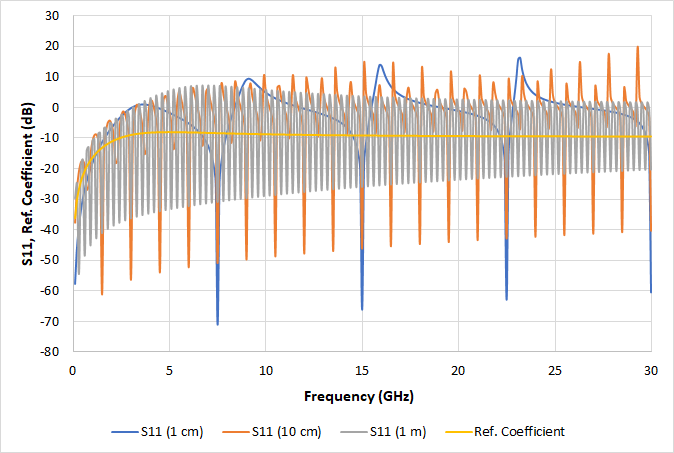
\includegraphics[width=0.5\textwidth]{figures/1pf_input.png}
            \caption{Comparison of S11 and reflection coefficient at the input to a load component with 1 pF input capacitance.}
        \end{figure}

        Đường truyền hoạt động giống như một khoang cộng hưởng điển hình\footnote{\href{https://resources.pcb.cadence.com/blog/2019-what-is-a-cavity-resonator-and-how-is-one-used-in-pcb-design}{\color{blue}What is a Cavity Resonator and How is One Used in PCB Design}} và có cấu trúc cộng hưởng khi đường truyền rất ngắn. khi đường truyền dài hơn, tổn thất bắt đầu chiếm ưu thế và cộng hưởng trong phổ S11 bắt đầu biến mất.\cite{cadence2021transmission}\par
        Khi kéo dài đường truyền ra vô cực, trở kháng đầu vào tại mỗi cổng giảm xuống (Phương trình \ref{eq:zin}). Đối với các đường truyền thực tế hoạt động ở tần số thực tế, cần phải mô tả hành vi tín hiệu theo trở kháng đầu vào và tham số S, đặc biệt là khi đường truyền ngắn.\cite{cadence2021transmission}\par